\ifdefined\ICLRLayout
\clearpage
% Auto-generated by paper/scripts/generate_overall_results_table.py.
% TFM rows come from the canonical summary_oof.csv files.
% TabDPT seven-shift Shared classification uses the audited Shared-v2 OOF overlay.
% Non-TFM rows come from the audited baseline CSV summary.
% The LimiX rows are emitted only after all completion audits pass.
\definecolor{tabaceSharedRow}{HTML}{EAF4FB}
\definecolor{tabaceSpecificRow}{HTML}{FFF4D6}
\definecolor{tabaceSharedText}{HTML}{0072B2}
\definecolor{tabaceSpecificText}{HTML}{D55E00}
\ifdefined\ICLRLayout
\begin{table}[H]
\else
\begin{table}[H]
\fi
  \caption{Overall performance on OpenML-CC18 classification and OpenML-CTR23
  regression tasks. The perturbation and shift blocks macro-average all
  nonzero strengths over five and seven families, respectively.}
  \label{tab:overall-performance}
  \centering
  \scriptsize
  \setlength{\tabcolsep}{2.0pt}
  \renewcommand{\arraystretch}{0.98}
  \begin{tabular}{@{}l*{12}{c}@{}}
    \toprule
    & \multicolumn{4}{c}{Clean}
    & \multicolumn{4}{c}{Five Perturbations (Avg.)}
    & \multicolumn{4}{c}{Seven Shifts (Avg.)} \\
    \cmidrule(lr){2-5}\cmidrule(lr){6-9}\cmidrule(lr){10-13}
    & \multicolumn{2}{c}{Classification} & \multicolumn{2}{c}{Regression}
    & \multicolumn{2}{c}{Classification} & \multicolumn{2}{c}{Regression}
    & \multicolumn{2}{c}{Classification} & \multicolumn{2}{c}{Regression} \\
    \cmidrule(lr){2-3}\cmidrule(lr){4-5}
    \cmidrule(lr){6-7}\cmidrule(lr){8-9}
    \cmidrule(lr){10-11}\cmidrule(lr){12-13}
    Method
    & Acc$\uparrow$ & AUC$\uparrow$ & $R^2\uparrow$ & nRMSE$\downarrow$
    & Acc$\uparrow$ & AUC$\uparrow$ & $R^2\uparrow$ & nRMSE$\downarrow$
    & Acc$\uparrow$ & AUC$\uparrow$ & $R^2\uparrow$ & nRMSE$\downarrow$ \\
    \midrule
    \multicolumn{13}{@{}l}{\textit{Non-TFM baselines}} \\
    LogReg/Ridge + HPO & 0.754 & 0.867 & 0.543 & 0.684 & 0.418 & 0.582 & -0.559 & 1.175 & 0.719 & 0.775 & -0.490 & 0.851 \\
    SVM/SVR + HPO & 0.777 & 0.879 & 0.492 & 0.703 & 0.449 & 0.611 & -0.872 & 1.255 & 0.757 & 0.793 & 0.010 & 0.873 \\
    kNN + HPO & 0.726 & 0.856 & 0.587 & 0.656 & 0.489 & 0.647 & -1.245 & 1.396 & 0.743 & 0.775 & 0.327 & 0.779 \\
    RF + HPO & 0.776 & 0.886 & 0.676 & 0.561 & 0.451 & 0.649 & -1.218 & 1.335 & 0.760 & 0.810 & 0.385 & 0.724 \\
    LightGBM + HPO & 0.776 & 0.884 & 0.697 & 0.529 & 0.463 & 0.639 & -1.215 & 1.337 & 0.759 & 0.796 & 0.350 & 0.736 \\
    CatBoost + HPO & 0.782 & 0.890 & 0.708 & 0.514 & 0.479 & 0.653 & -1.372 & 1.368 & 0.770 & 0.811 & 0.381 & 0.711 \\
    XGBoost + HPO & 0.774 & 0.885 & 0.702 & 0.525 & 0.455 & 0.640 & -1.323 & 1.359 & 0.751 & 0.796 & 0.278 & 0.767 \\
    MLP + HPO & 0.729 & 0.858 & 0.583 & 0.568 & 0.435 & 0.604 & -1.007 & 1.272 & 0.741 & 0.767 & 0.066 & 0.828 \\
    FT-Transformer & 0.745 & 0.861 & 0.657 & 0.568 & 0.456 & 0.619 & -1.256 & 1.353 & 0.716 & 0.765 & 0.210 & 0.822 \\
    TabM & 0.735 & 0.866 & 0.655 & 0.577 & 0.454 & 0.614 & -1.100 & 1.324 & 0.699 & 0.743 & 0.212 & 0.811 \\
    TabulaRNN & 0.722 & 0.856 & 0.580 & 0.648 & 0.454 & 0.625 & -0.851 & 1.270 & 0.718 & 0.754 & 0.205 & 0.845 \\
    MambaTab & 0.748 & 0.869 & 0.663 & 0.564 & 0.434 & 0.602 & -0.824 & 1.230 & 0.751 & 0.784 & 0.279 & 0.761 \\
    RealMLP & 0.762 & 0.872 & 0.694 & 0.527 & 0.448 & 0.614 & -1.258 & 1.326 & 0.758 & 0.793 & 0.240 & 0.749 \\
    \midrule
    LimiX-2M & 0.796 & 0.896 & 0.724 & 0.494 & 0.475 & 0.657 & -1.141 & 1.277 & 0.781 & 0.831 & 0.385 & 0.689 \\
    \rowcolor{tabaceSharedRow}
    \textcolor{tabaceSharedText}{\textbf{+ \method{}-shared}} & \textcolor{tabaceSharedText}{\textbf{0.796}} & \textcolor{tabaceSharedText}{\textbf{0.896}} & \textcolor{tabaceSharedText}{\textbf{0.725}} & \textcolor{tabaceSharedText}{\textbf{0.493}} & \textcolor{tabaceSharedText}{\textbf{0.542}} & \textcolor{tabaceSharedText}{\textbf{0.716}} & \textcolor{tabaceSharedText}{\textbf{-0.173}} & \textcolor{tabaceSharedText}{\textbf{1.059}} & \textcolor{tabaceSharedText}{\textbf{0.784}} & \textcolor{tabaceSharedText}{\textbf{0.835}} & \textcolor{tabaceSharedText}{\textbf{0.498}} & \textcolor{tabaceSharedText}{\textbf{0.659}} \\
    \rowcolor{tabaceSpecificRow}
    \textcolor{tabaceSpecificText}{\textbf{+ \method{}-specific}} & \textcolor{tabaceSpecificText}{\textbf{0.796}} & \textcolor{tabaceSpecificText}{\textbf{0.896}} & \textcolor{tabaceSpecificText}{\textbf{0.725}} & \textcolor{tabaceSpecificText}{\textbf{0.493}} & \textcolor{tabaceSpecificText}{\textbf{0.628}} & \textcolor{tabaceSpecificText}{\textbf{0.769}} & \textcolor{tabaceSpecificText}{\textbf{0.053}} & \textcolor{tabaceSpecificText}{\textbf{0.947}} & \textcolor{tabaceSpecificText}{\textbf{0.804}} & \textcolor{tabaceSpecificText}{\textbf{0.847}} & \textcolor{tabaceSpecificText}{\textbf{0.629}} & \textcolor{tabaceSpecificText}{\textbf{0.563}} \\
    \midrule
    TabICL-v2 & 0.804 & 0.901 & 0.739 & 0.476 & 0.494 & 0.676 & -1.077 & 1.270 & 0.763 & 0.826 & 0.273 & 0.730 \\
    \rowcolor{tabaceSharedRow}
    \textcolor{tabaceSharedText}{\textbf{+ \method{}-shared}} & \textcolor{tabaceSharedText}{\textbf{0.804}} & \textcolor{tabaceSharedText}{\textbf{0.901}} & \textcolor{tabaceSharedText}{\textbf{0.738}} & \textcolor{tabaceSharedText}{\textbf{0.478}} & \textcolor{tabaceSharedText}{\textbf{0.575}} & \textcolor{tabaceSharedText}{\textbf{0.720}} & \textcolor{tabaceSharedText}{\textbf{0.363}} & \textcolor{tabaceSharedText}{\textbf{0.783}} & \textcolor{tabaceSharedText}{\textbf{0.772}} & \textcolor{tabaceSharedText}{\textbf{0.831}} & \textcolor{tabaceSharedText}{\textbf{0.467}} & \textcolor{tabaceSharedText}{\textbf{0.659}} \\
    \rowcolor{tabaceSpecificRow}
    \textcolor{tabaceSpecificText}{\textbf{+ \method{}-specific}} & \textcolor{tabaceSpecificText}{\textbf{0.804}} & \textcolor{tabaceSpecificText}{\textbf{0.900}} & \textcolor{tabaceSpecificText}{\textbf{0.738}} & \textcolor{tabaceSpecificText}{\textbf{0.476}} & \textcolor{tabaceSpecificText}{\textbf{0.610}} & \textcolor{tabaceSpecificText}{\textbf{0.752}} & \textcolor{tabaceSpecificText}{\textbf{0.485}} & \textcolor{tabaceSpecificText}{\textbf{0.708}} & \textcolor{tabaceSpecificText}{\textbf{0.805}} & \textcolor{tabaceSpecificText}{\textbf{0.854}} & \textcolor{tabaceSpecificText}{\textbf{0.655}} & \textcolor{tabaceSpecificText}{\textbf{0.535}} \\
    \midrule
    TabPFN-v3 & 0.793 & 0.893 & 0.739 & 0.476 & 0.457 & 0.636 & -1.253 & 1.313 & 0.758 & 0.809 & 0.426 & 0.669 \\
    \rowcolor{tabaceSharedRow}
    \textcolor{tabaceSharedText}{\textbf{+ \method{}-shared}} & \textcolor{tabaceSharedText}{\textbf{0.792}} & \textcolor{tabaceSharedText}{\textbf{0.893}} & \textcolor{tabaceSharedText}{\textbf{0.739}} & \textcolor{tabaceSharedText}{\textbf{0.480}} & \textcolor{tabaceSharedText}{\textbf{0.553}} & \textcolor{tabaceSharedText}{\textbf{0.697}} & \textcolor{tabaceSharedText}{\textbf{0.237}} & \textcolor{tabaceSharedText}{\textbf{0.834}} & \textcolor{tabaceSharedText}{\textbf{0.770}} & \textcolor{tabaceSharedText}{\textbf{0.817}} & \textcolor{tabaceSharedText}{\textbf{0.460}} & \textcolor{tabaceSharedText}{\textbf{0.656}} \\
    \rowcolor{tabaceSpecificRow}
    \textcolor{tabaceSpecificText}{\textbf{+ \method{}-specific}} & \textcolor{tabaceSpecificText}{\textbf{0.792}} & \textcolor{tabaceSpecificText}{\textbf{0.893}} & \textcolor{tabaceSpecificText}{\textbf{0.739}} & \textcolor{tabaceSpecificText}{\textbf{0.477}} & \textcolor{tabaceSpecificText}{\textbf{0.593}} & \textcolor{tabaceSpecificText}{\textbf{0.739}} & \textcolor{tabaceSpecificText}{\textbf{0.588}} & \textcolor{tabaceSpecificText}{\textbf{0.635}} & \textcolor{tabaceSpecificText}{\textbf{0.788}} & \textcolor{tabaceSpecificText}{\textbf{0.835}} & \textcolor{tabaceSpecificText}{\textbf{0.620}} & \textcolor{tabaceSpecificText}{\textbf{0.565}} \\
    \midrule
    TabDPT v1.2 & 0.779 & 0.891 & 0.731 & 0.488 & 0.448 & 0.631 & -1.152 & 1.300 & 0.774 & 0.821 & 0.514 & 0.633 \\
    \rowcolor{tabaceSharedRow}
    \textcolor{tabaceSharedText}{\textbf{+ \method{}-shared}} & \textcolor{tabaceSharedText}{\textbf{0.779}} & \textcolor{tabaceSharedText}{\textbf{0.891}} & \textcolor{tabaceSharedText}{\textbf{0.730}} & \textcolor{tabaceSharedText}{\textbf{0.491}} & \textcolor{tabaceSharedText}{\textbf{0.548}} & \textcolor{tabaceSharedText}{\textbf{0.694}} & \textcolor{tabaceSharedText}{\textbf{0.329}} & \textcolor{tabaceSharedText}{\textbf{0.803}} & \textcolor{tabaceSharedText}{\textbf{0.781}} & \textcolor{tabaceSharedText}{\textbf{0.831}} & \textcolor{tabaceSharedText}{\textbf{0.547}} & \textcolor{tabaceSharedText}{\textbf{0.614}} \\
    \rowcolor{tabaceSpecificRow}
    \textcolor{tabaceSpecificText}{\textbf{+ \method{}-specific}} & \textcolor{tabaceSpecificText}{\textbf{0.779}} & \textcolor{tabaceSpecificText}{\textbf{0.891}} & \textcolor{tabaceSpecificText}{\textbf{0.730}} & \textcolor{tabaceSpecificText}{\textbf{0.488}} & \textcolor{tabaceSpecificText}{\textbf{0.600}} & \textcolor{tabaceSpecificText}{\textbf{0.746}} & \textcolor{tabaceSpecificText}{\textbf{0.443}} & \textcolor{tabaceSpecificText}{\textbf{0.733}} & \textcolor{tabaceSpecificText}{\textbf{0.805}} & \textcolor{tabaceSpecificText}{\textbf{0.846}} & \textcolor{tabaceSpecificText}{\textbf{0.610}} & \textcolor{tabaceSpecificText}{\textbf{0.572}} \\
    \bottomrule
  \end{tabular}
\ifdefined\ICLRLayout
\end{table}
\else
\end{table}
\fi

\else
\begin{figure}[H]
  \centering
  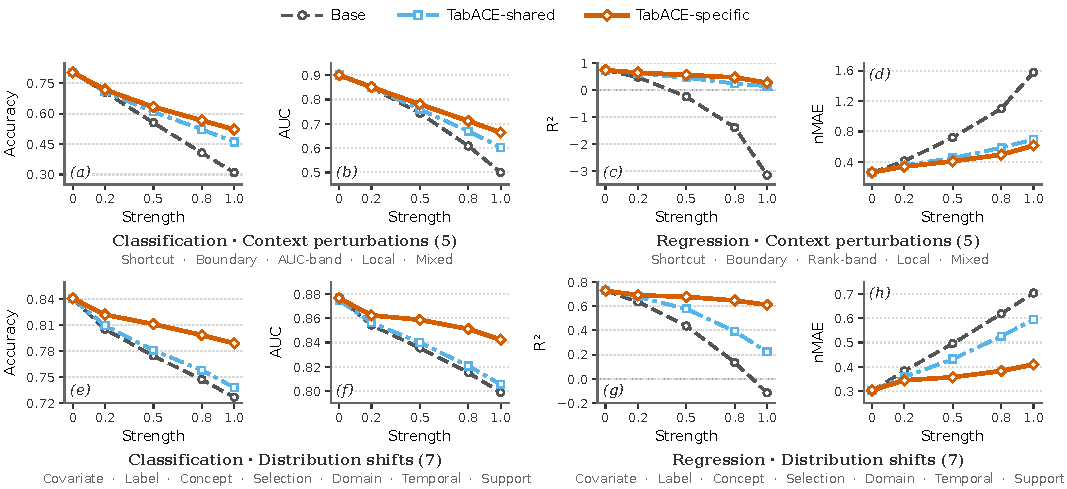
\includegraphics[width=\textwidth]{figures/tabace_strength_comparison.pdf}
  \caption{Performance across problem strengths on OpenML benchmarks.
  Classification panels use OpenML-CC18 and regression panels use
  OpenML-CTR23. The first row macro-averages five controlled context
  perturbations; the second macro-averages seven distribution shifts.}
  \label{fig:semisynthetic-strength}
\end{figure}

\clearpage
% Auto-generated by paper/scripts/generate_overall_results_table.py.
% TFM rows come from the canonical summary_oof.csv files.
% TabDPT seven-shift Shared classification uses the audited Shared-v2 OOF overlay.
% Non-TFM rows come from the audited baseline CSV summary.
% The LimiX rows are emitted only after all completion audits pass.
\definecolor{tabaceSharedRow}{HTML}{EAF4FB}
\definecolor{tabaceSpecificRow}{HTML}{FFF4D6}
\definecolor{tabaceSharedText}{HTML}{0072B2}
\definecolor{tabaceSpecificText}{HTML}{D55E00}
\ifdefined\ICLRLayout
\begin{table}[H]
\else
\begin{table}[H]
\fi
  \caption{Overall performance on OpenML-CC18 classification and OpenML-CTR23
  regression tasks. The perturbation and shift blocks macro-average all
  nonzero strengths over five and seven families, respectively.}
  \label{tab:overall-performance}
  \centering
  \scriptsize
  \setlength{\tabcolsep}{2.0pt}
  \renewcommand{\arraystretch}{0.98}
  \begin{tabular}{@{}l*{12}{c}@{}}
    \toprule
    & \multicolumn{4}{c}{Clean}
    & \multicolumn{4}{c}{Five Perturbations (Avg.)}
    & \multicolumn{4}{c}{Seven Shifts (Avg.)} \\
    \cmidrule(lr){2-5}\cmidrule(lr){6-9}\cmidrule(lr){10-13}
    & \multicolumn{2}{c}{Classification} & \multicolumn{2}{c}{Regression}
    & \multicolumn{2}{c}{Classification} & \multicolumn{2}{c}{Regression}
    & \multicolumn{2}{c}{Classification} & \multicolumn{2}{c}{Regression} \\
    \cmidrule(lr){2-3}\cmidrule(lr){4-5}
    \cmidrule(lr){6-7}\cmidrule(lr){8-9}
    \cmidrule(lr){10-11}\cmidrule(lr){12-13}
    Method
    & Acc$\uparrow$ & AUC$\uparrow$ & $R^2\uparrow$ & nRMSE$\downarrow$
    & Acc$\uparrow$ & AUC$\uparrow$ & $R^2\uparrow$ & nRMSE$\downarrow$
    & Acc$\uparrow$ & AUC$\uparrow$ & $R^2\uparrow$ & nRMSE$\downarrow$ \\
    \midrule
    \multicolumn{13}{@{}l}{\textit{Non-TFM baselines}} \\
    LogReg/Ridge + HPO & 0.754 & 0.867 & 0.543 & 0.684 & 0.418 & 0.582 & -0.559 & 1.175 & 0.719 & 0.775 & -0.490 & 0.851 \\
    SVM/SVR + HPO & 0.777 & 0.879 & 0.492 & 0.703 & 0.449 & 0.611 & -0.872 & 1.255 & 0.757 & 0.793 & 0.010 & 0.873 \\
    kNN + HPO & 0.726 & 0.856 & 0.587 & 0.656 & 0.489 & 0.647 & -1.245 & 1.396 & 0.743 & 0.775 & 0.327 & 0.779 \\
    RF + HPO & 0.776 & 0.886 & 0.676 & 0.561 & 0.451 & 0.649 & -1.218 & 1.335 & 0.760 & 0.810 & 0.385 & 0.724 \\
    LightGBM + HPO & 0.776 & 0.884 & 0.697 & 0.529 & 0.463 & 0.639 & -1.215 & 1.337 & 0.759 & 0.796 & 0.350 & 0.736 \\
    CatBoost + HPO & 0.782 & 0.890 & 0.708 & 0.514 & 0.479 & 0.653 & -1.372 & 1.368 & 0.770 & 0.811 & 0.381 & 0.711 \\
    XGBoost + HPO & 0.774 & 0.885 & 0.702 & 0.525 & 0.455 & 0.640 & -1.323 & 1.359 & 0.751 & 0.796 & 0.278 & 0.767 \\
    MLP + HPO & 0.729 & 0.858 & 0.583 & 0.568 & 0.435 & 0.604 & -1.007 & 1.272 & 0.741 & 0.767 & 0.066 & 0.828 \\
    FT-Transformer & 0.745 & 0.861 & 0.657 & 0.568 & 0.456 & 0.619 & -1.256 & 1.353 & 0.716 & 0.765 & 0.210 & 0.822 \\
    TabM & 0.735 & 0.866 & 0.655 & 0.577 & 0.454 & 0.614 & -1.100 & 1.324 & 0.699 & 0.743 & 0.212 & 0.811 \\
    TabulaRNN & 0.722 & 0.856 & 0.580 & 0.648 & 0.454 & 0.625 & -0.851 & 1.270 & 0.718 & 0.754 & 0.205 & 0.845 \\
    MambaTab & 0.748 & 0.869 & 0.663 & 0.564 & 0.434 & 0.602 & -0.824 & 1.230 & 0.751 & 0.784 & 0.279 & 0.761 \\
    RealMLP & 0.762 & 0.872 & 0.694 & 0.527 & 0.448 & 0.614 & -1.258 & 1.326 & 0.758 & 0.793 & 0.240 & 0.749 \\
    \midrule
    LimiX-2M & 0.796 & 0.896 & 0.724 & 0.494 & 0.475 & 0.657 & -1.141 & 1.277 & 0.781 & 0.831 & 0.385 & 0.689 \\
    \rowcolor{tabaceSharedRow}
    \textcolor{tabaceSharedText}{\textbf{+ \method{}-shared}} & \textcolor{tabaceSharedText}{\textbf{0.796}} & \textcolor{tabaceSharedText}{\textbf{0.896}} & \textcolor{tabaceSharedText}{\textbf{0.725}} & \textcolor{tabaceSharedText}{\textbf{0.493}} & \textcolor{tabaceSharedText}{\textbf{0.542}} & \textcolor{tabaceSharedText}{\textbf{0.716}} & \textcolor{tabaceSharedText}{\textbf{-0.173}} & \textcolor{tabaceSharedText}{\textbf{1.059}} & \textcolor{tabaceSharedText}{\textbf{0.784}} & \textcolor{tabaceSharedText}{\textbf{0.835}} & \textcolor{tabaceSharedText}{\textbf{0.498}} & \textcolor{tabaceSharedText}{\textbf{0.659}} \\
    \rowcolor{tabaceSpecificRow}
    \textcolor{tabaceSpecificText}{\textbf{+ \method{}-specific}} & \textcolor{tabaceSpecificText}{\textbf{0.796}} & \textcolor{tabaceSpecificText}{\textbf{0.896}} & \textcolor{tabaceSpecificText}{\textbf{0.725}} & \textcolor{tabaceSpecificText}{\textbf{0.493}} & \textcolor{tabaceSpecificText}{\textbf{0.628}} & \textcolor{tabaceSpecificText}{\textbf{0.769}} & \textcolor{tabaceSpecificText}{\textbf{0.053}} & \textcolor{tabaceSpecificText}{\textbf{0.947}} & \textcolor{tabaceSpecificText}{\textbf{0.804}} & \textcolor{tabaceSpecificText}{\textbf{0.847}} & \textcolor{tabaceSpecificText}{\textbf{0.629}} & \textcolor{tabaceSpecificText}{\textbf{0.563}} \\
    \midrule
    TabICL-v2 & 0.804 & 0.901 & 0.739 & 0.476 & 0.494 & 0.676 & -1.077 & 1.270 & 0.763 & 0.826 & 0.273 & 0.730 \\
    \rowcolor{tabaceSharedRow}
    \textcolor{tabaceSharedText}{\textbf{+ \method{}-shared}} & \textcolor{tabaceSharedText}{\textbf{0.804}} & \textcolor{tabaceSharedText}{\textbf{0.901}} & \textcolor{tabaceSharedText}{\textbf{0.738}} & \textcolor{tabaceSharedText}{\textbf{0.478}} & \textcolor{tabaceSharedText}{\textbf{0.575}} & \textcolor{tabaceSharedText}{\textbf{0.720}} & \textcolor{tabaceSharedText}{\textbf{0.363}} & \textcolor{tabaceSharedText}{\textbf{0.783}} & \textcolor{tabaceSharedText}{\textbf{0.772}} & \textcolor{tabaceSharedText}{\textbf{0.831}} & \textcolor{tabaceSharedText}{\textbf{0.467}} & \textcolor{tabaceSharedText}{\textbf{0.659}} \\
    \rowcolor{tabaceSpecificRow}
    \textcolor{tabaceSpecificText}{\textbf{+ \method{}-specific}} & \textcolor{tabaceSpecificText}{\textbf{0.804}} & \textcolor{tabaceSpecificText}{\textbf{0.900}} & \textcolor{tabaceSpecificText}{\textbf{0.738}} & \textcolor{tabaceSpecificText}{\textbf{0.476}} & \textcolor{tabaceSpecificText}{\textbf{0.610}} & \textcolor{tabaceSpecificText}{\textbf{0.752}} & \textcolor{tabaceSpecificText}{\textbf{0.485}} & \textcolor{tabaceSpecificText}{\textbf{0.708}} & \textcolor{tabaceSpecificText}{\textbf{0.805}} & \textcolor{tabaceSpecificText}{\textbf{0.854}} & \textcolor{tabaceSpecificText}{\textbf{0.655}} & \textcolor{tabaceSpecificText}{\textbf{0.535}} \\
    \midrule
    TabPFN-v3 & 0.793 & 0.893 & 0.739 & 0.476 & 0.457 & 0.636 & -1.253 & 1.313 & 0.758 & 0.809 & 0.426 & 0.669 \\
    \rowcolor{tabaceSharedRow}
    \textcolor{tabaceSharedText}{\textbf{+ \method{}-shared}} & \textcolor{tabaceSharedText}{\textbf{0.792}} & \textcolor{tabaceSharedText}{\textbf{0.893}} & \textcolor{tabaceSharedText}{\textbf{0.739}} & \textcolor{tabaceSharedText}{\textbf{0.480}} & \textcolor{tabaceSharedText}{\textbf{0.553}} & \textcolor{tabaceSharedText}{\textbf{0.697}} & \textcolor{tabaceSharedText}{\textbf{0.237}} & \textcolor{tabaceSharedText}{\textbf{0.834}} & \textcolor{tabaceSharedText}{\textbf{0.770}} & \textcolor{tabaceSharedText}{\textbf{0.817}} & \textcolor{tabaceSharedText}{\textbf{0.460}} & \textcolor{tabaceSharedText}{\textbf{0.656}} \\
    \rowcolor{tabaceSpecificRow}
    \textcolor{tabaceSpecificText}{\textbf{+ \method{}-specific}} & \textcolor{tabaceSpecificText}{\textbf{0.792}} & \textcolor{tabaceSpecificText}{\textbf{0.893}} & \textcolor{tabaceSpecificText}{\textbf{0.739}} & \textcolor{tabaceSpecificText}{\textbf{0.477}} & \textcolor{tabaceSpecificText}{\textbf{0.593}} & \textcolor{tabaceSpecificText}{\textbf{0.739}} & \textcolor{tabaceSpecificText}{\textbf{0.588}} & \textcolor{tabaceSpecificText}{\textbf{0.635}} & \textcolor{tabaceSpecificText}{\textbf{0.788}} & \textcolor{tabaceSpecificText}{\textbf{0.835}} & \textcolor{tabaceSpecificText}{\textbf{0.620}} & \textcolor{tabaceSpecificText}{\textbf{0.565}} \\
    \midrule
    TabDPT v1.2 & 0.779 & 0.891 & 0.731 & 0.488 & 0.448 & 0.631 & -1.152 & 1.300 & 0.774 & 0.821 & 0.514 & 0.633 \\
    \rowcolor{tabaceSharedRow}
    \textcolor{tabaceSharedText}{\textbf{+ \method{}-shared}} & \textcolor{tabaceSharedText}{\textbf{0.779}} & \textcolor{tabaceSharedText}{\textbf{0.891}} & \textcolor{tabaceSharedText}{\textbf{0.730}} & \textcolor{tabaceSharedText}{\textbf{0.491}} & \textcolor{tabaceSharedText}{\textbf{0.548}} & \textcolor{tabaceSharedText}{\textbf{0.694}} & \textcolor{tabaceSharedText}{\textbf{0.329}} & \textcolor{tabaceSharedText}{\textbf{0.803}} & \textcolor{tabaceSharedText}{\textbf{0.781}} & \textcolor{tabaceSharedText}{\textbf{0.831}} & \textcolor{tabaceSharedText}{\textbf{0.547}} & \textcolor{tabaceSharedText}{\textbf{0.614}} \\
    \rowcolor{tabaceSpecificRow}
    \textcolor{tabaceSpecificText}{\textbf{+ \method{}-specific}} & \textcolor{tabaceSpecificText}{\textbf{0.779}} & \textcolor{tabaceSpecificText}{\textbf{0.891}} & \textcolor{tabaceSpecificText}{\textbf{0.730}} & \textcolor{tabaceSpecificText}{\textbf{0.488}} & \textcolor{tabaceSpecificText}{\textbf{0.600}} & \textcolor{tabaceSpecificText}{\textbf{0.746}} & \textcolor{tabaceSpecificText}{\textbf{0.443}} & \textcolor{tabaceSpecificText}{\textbf{0.733}} & \textcolor{tabaceSpecificText}{\textbf{0.805}} & \textcolor{tabaceSpecificText}{\textbf{0.846}} & \textcolor{tabaceSpecificText}{\textbf{0.610}} & \textcolor{tabaceSpecificText}{\textbf{0.572}} \\
    \bottomrule
  \end{tabular}
\ifdefined\ICLRLayout
\end{table}
\else
\end{table}
\fi

\fi

\section{Experiments}
\label{sec:experiments}

\subsection{Experimental Setup}
\label{sec:experimental_setup}

\paragraph{Evaluation tracks.}
We evaluate TabACE on public OpenML benchmarks and fully synthetic data. The
OpenML track draws classification tasks from OpenML-CC18~\citep{bischl2021openml}
and regression tasks from OpenML-CTR23~\citep{fischer2023openmlctr23}. Controlled
changes use five-fold dataset-level out-of-fold (OOF) evaluation: policies are
fitted on the other four folds and fixed for held-out datasets. Strength zero
leaves the context and input unchanged. Controlled data-generating processes in
the synthetic track isolate problem family and strength.

\paragraph{Problems and configurations.}
Both tracks cover five source-context perturbations (Shortcut, Boundary,
AUC/Rank-band, Local, and Mixed) and seven distribution shifts (Covariate,
Label, Concept, Selection, Domain, Temporal, and Support) at strengths $0$,
$0.2$, $0.5$, $0.8$, and $1.0$. Base is the frozen backbone without context
ensembling. Shared uses a fixed context bank across the predefined changes,
whereas Specific selects and fuses candidates using a change family specified
before target inference. All secondary experiments use frozen TabICL-v2 unless
another predictor is named. Base denotes its unmodified prediction. The appendix
lists the operators and context layouts.

% Register this float before the final setup paragraphs so that the arXiv
% layout places it at the top of page 7.  The ICLR layout inserts the same
% figure at the corresponding results subsection instead.
\ifdefined\ICLRLayout\else
\clearpage
\begin{figure}[H]
  \centering
  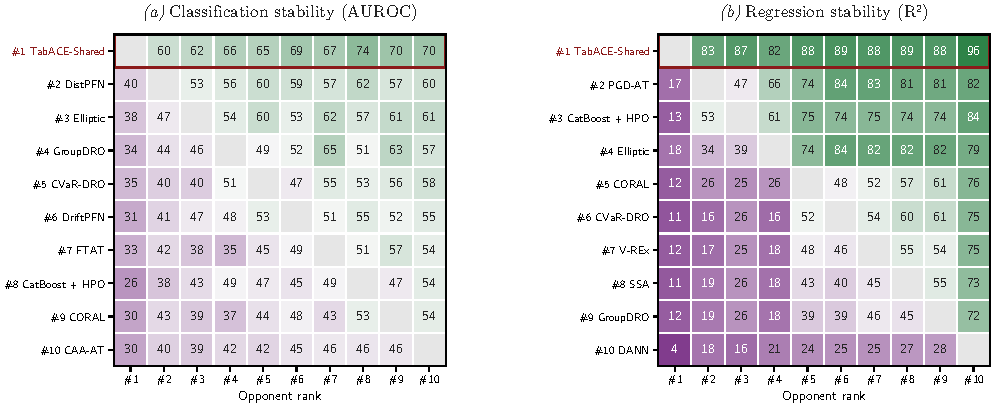
\includegraphics[width=0.88\textwidth]{figures/tabace_synthetic_stability.pdf}
  \caption{Pairwise stability over 180 aligned seed--DGP--scenario units.
  Classification uses chance-adjusted AUROC-margin degradation and regression
  uses normalized $R^2$ degradation. Cells show how often the row method has
  the smaller drop; differences within $0.001$ are ties.}
  \label{fig:synthetic-stability}
\end{figure}

\begin{figure}[H]
  \centering
  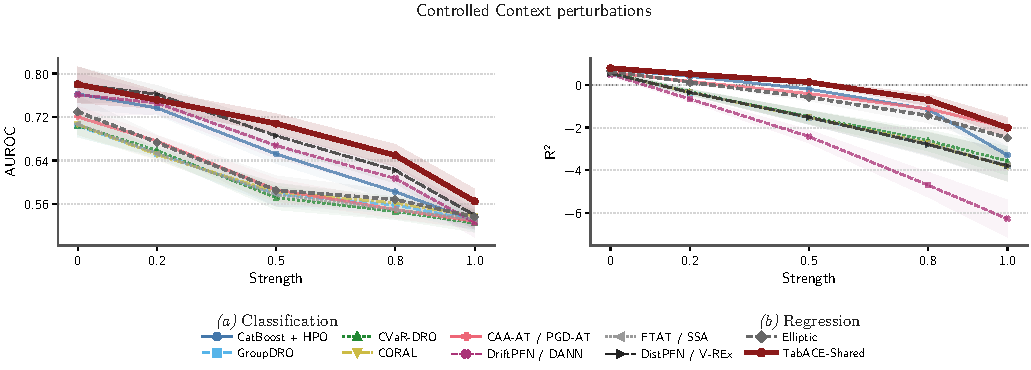
\includegraphics[width=0.94\textwidth]{figures/tabace_controlled_response.pdf}
  \caption{Fully synthetic response to controlled context perturbations.
  Panels report classification AUROC and regression $R^2$; curves pool
  aligned units over five perturbation families and bands show 95\% bootstrap
  intervals.}
  \label{fig:synthetic-controlled-response}
\end{figure}
\fi

\paragraph{Task and metrics.}
We report Accuracy and AUROC for classification and $R^2$, nMAE, and nRMSE for
regression. Robustness rankings and strength-response plots use AUROC and
$R^2$, respectively.

\paragraph{Baselines.}
The OpenML study compares tuned conventional, tree-based, neural, and frozen
foundation-model predictors, including the LimiX-2M checkpoint (hereafter
LimiX)~\citep{wang2026limix2m}. The synthetic study
compares robust-learning, adversarial-training, and distribution-adaptation
baselines. The appendix lists all methods and their task applicability, including
the compatibility protocol used to cover the complete OpenML suites with LimiX.

\ifdefined\ICLRLayout
\clearpage
\begin{figure}[H]
  \centering
  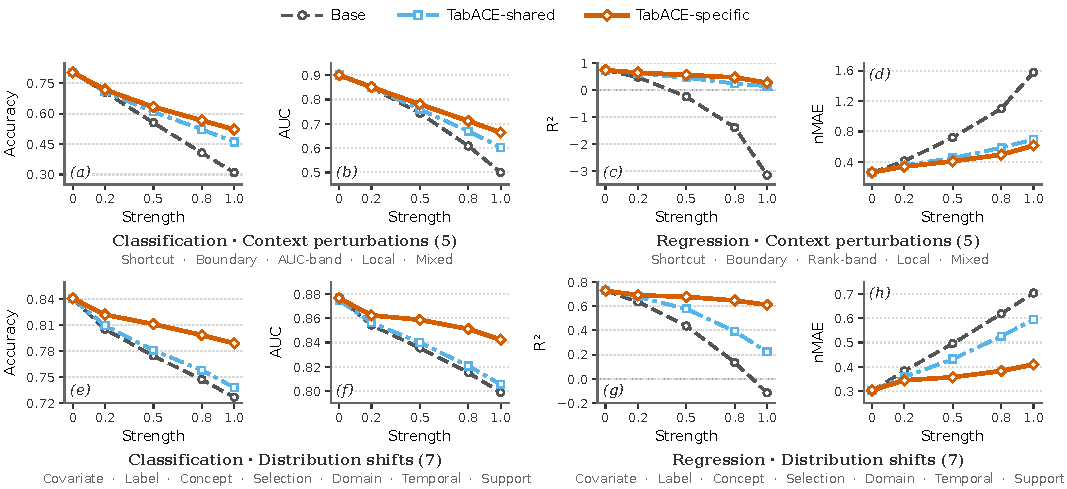
\includegraphics[width=\textwidth]{figures/tabace_strength_comparison.pdf}
  \caption{Performance across problem strengths on OpenML benchmarks.
  Classification panels use OpenML-CC18 and regression panels use
  OpenML-CTR23. The first row macro-averages five controlled context
  perturbations; the second macro-averages seven distribution shifts.}
  \label{fig:semisynthetic-strength}
\end{figure}
\fi

\paragraph{Selection protocol.}
Within each outer fold, context configurations, branch weights, and integration
parameters are fitted on calibration episodes from the other four dataset folds
and fixed before held-out-dataset evaluation. These episodes cover the registered
conditions, but strength is not supplied to the fitted policy or held-out
inference. All methods share the same outer folds and evaluation samples, and
held-out target labels are used only for final metrics.

% Keep the two compact tables and the inference-cost figure together at the
% top of arXiv page 8, after the page-7 figures and setup text.
\ifdefined\ICLRLayout\else
\clearpage
\providecolor{revisionblue}{RGB}{25,55,135}
\definecolor{sharedblue}{RGB}{31,84,147}
\definecolor{specificred}{RGB}{213,94,0}

\begin{table}[H]
  \centering
  \begin{minipage}[t]{0.61\textwidth}
    \vspace{0pt}
    \centering
    \caption{ID and OOD Accuracy under natural geographic and temporal shifts.}
    \label{tab:natural-shifts}
    \small
    \setlength{\tabcolsep}{4.0pt}
    \renewcommand{\arraystretch}{1.02}
    \begin{tabular}{@{}llccc@{}}
      \toprule
      Method & Domain & Employment & Income & TravelTime \\
      \midrule
      \multicolumn{5}{@{}l}{\textit{Geographic: California $\rightarrow$ Michigan (2018)}} \\
      Base & ID  & 0.7922 & 0.7888 & 0.5912 \\
           & OOD & 0.8043 & 0.7655 & 0.5472 \\
      Shared & ID
        & \textcolor{revisionblue}{0.7952} & \textcolor{revisionblue}{0.8118}
        & \textcolor{revisionblue}{0.6225} \\
           & OOD
        & \textcolor{revisionblue}{0.8106} & \textcolor{revisionblue}{0.7823}
        & \textcolor{revisionblue}{0.5818} \\
      Specific & ID
        & \textcolor{revisionblue}{\textbf{0.8089}}
        & \textcolor{revisionblue}{\textbf{0.8201}}
        & \textcolor{revisionblue}{\textbf{0.6569}} \\
           & OOD
        & \textcolor{revisionblue}{\textbf{0.8245}}
        & \textcolor{revisionblue}{\textbf{0.7914}}
        & \textcolor{revisionblue}{\textbf{0.6012}} \\
      \addlinespace[2pt]
      \multicolumn{5}{@{}l}{\textit{Temporal: California 2014 $\rightarrow$ 2018}} \\
      Base & ID  & 0.7704 & 0.7926 & 0.5951 \\
           & OOD & 0.7847 & 0.7844 & 0.5908 \\
      Shared & ID
        & \textcolor{revisionblue}{0.7861} & \textcolor{revisionblue}{0.8126}
        & \textcolor{revisionblue}{0.6237} \\
           & OOD
        & \textcolor{revisionblue}{0.7922} & \textcolor{revisionblue}{0.8000}
        & \textcolor{revisionblue}{0.6045} \\
      Specific & ID
        & \textcolor{revisionblue}{\textbf{0.7994}}
        & \textcolor{revisionblue}{\textbf{0.8240}}
        & \textcolor{revisionblue}{\textbf{0.6526}} \\
           & OOD
        & \textcolor{revisionblue}{\textbf{0.8030}}
        & \textcolor{revisionblue}{\textbf{0.8106}}
        & \textcolor{revisionblue}{\textbf{0.6350}} \\
      \bottomrule
    \end{tabular}
  \end{minipage}\hfill
  \begin{minipage}[t]{0.36\textwidth}
    \vspace{0pt}
    \centering
    \caption{Gains over each unmodified conventional predictor from context ensembling.}
    \label{tab:traditional-backbone-gains}
    \small
    \setlength{\tabcolsep}{4.0pt}
    \renewcommand{\arraystretch}{1.02}
    \begin{tabular}{@{}lcc@{}}
      \toprule
      \multicolumn{3}{c}{Classification: $\Delta$Accuracy $\uparrow$} \\
      \cmidrule(lr){1-3}
      Predictor & Shared & Specific \\
      \midrule
      kNN & \textcolor{sharedblue}{+0.0167}
        & \textcolor{specificred}{\textbf{+0.0227}} \\
      Logistic & \textcolor{sharedblue}{+0.0069}
        & \textcolor{specificred}{\textbf{+0.0287}} \\
      CatBoost & \textcolor{sharedblue}{+0.0145}
        & \textcolor{specificred}{\textbf{+0.0287}} \\
      MLP & \textcolor{sharedblue}{+0.0107}
        & \textcolor{specificred}{\textbf{+0.0285}} \\
      \addlinespace[5pt]
      \multicolumn{3}{c}{Regression: $\Delta R^2$ $\uparrow$} \\
      \cmidrule(lr){1-3}
      Predictor & Shared & Specific \\
      \midrule
      kNN & \textcolor{sharedblue}{+0.0203}
        & \textcolor{specificred}{\textbf{+0.0654}} \\
      Ridge & \textcolor{sharedblue}{+0.1425}
        & \textcolor{specificred}{\textbf{+0.1966}} \\
      CatBoost & \textcolor{sharedblue}{+0.1279}
        & \textcolor{specificred}{\textbf{+0.1740}} \\
      MLP & \textcolor{sharedblue}{+0.0499}
        & \textcolor{specificred}{\textbf{+0.1645}} \\
      \bottomrule
    \end{tabular}
  \end{minipage}
\end{table}


\begin{figure}[H]
  \centering
  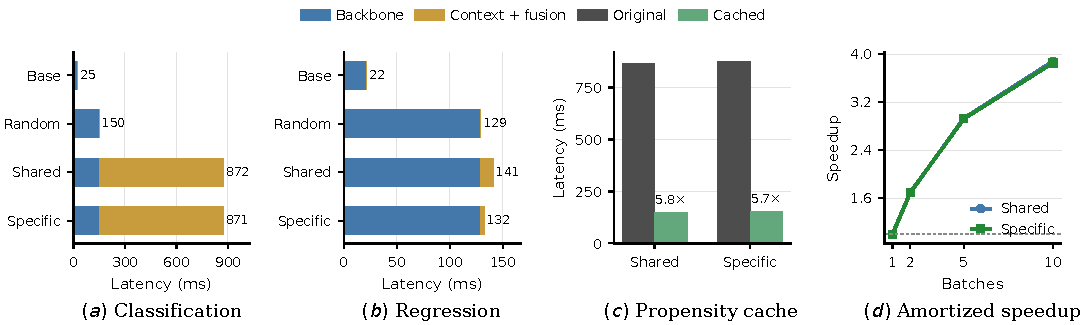
\includegraphics[width=0.96\textwidth]{figures/tabace_inference_cost_ablation.pdf}
  \caption{Inference-cost ablation for the fixed five-context Shared bank and a
  separately evaluated Base branch. Panels (a--b) decompose median latency;
  (c) compares original and cached inference; (d) includes the one-time cache
  setup in the amortized speedup.}
  \label{fig:inference-cost}
\end{figure}
\fi
